\chapter{Lebensformen}
\subsection{Humanoide}
\begin{itemize}
	\item Sämtliche (derzeit bekannte) normale Menschenarten haben sich aus den entsprechenden (gleichen) "Affen" entwickelt. Wesen wie Argonier oder Kajits gibt es bei uns also nicht.
	\item Die Arten sind immer wie bei der typischen Artenbildung in exklusiven Gebieten entstanden
	also es erfolgte eine allgemeine gleiche Entwicklung und manche Arten waren dann abgeschieden von anderen besonderen Umweltbedingungen ausgesetzt und haben deshalb bestimmte Merkmale neu entwickelt oder rückentwickelt
	\item die im folgenden vorgestellten Arten sind teilweise nur Anregungen und Beispiele und müssen nicht im Spiel enthalten sein. Ebenso können sie einfach Teil der Welt und unserer Gegend nicht oder nur durch Geschichten bekannt sein. Ist jedoch für später durchaus wichtig :smiley:
	\item Das heißt auch, dass die Menschenarten keine Federn oder Schuppen haben -- wenn die nicht irgendwie begründbar sind (max. Schuppen). Denn Federn sind was rein von den Vögeln, die mit den Säugern nix zu tun haben
	mit Hörnern bzw. Horn an sich kann natürlich viel gearbeitet werden
	\item natürlich kann es sein, dass wir durch besondere Umweltgeschehnisse mit viel Magie auch noch andere Arten haben, die sind dann aber "`unnatürlich"'
\end{itemize}

\paragraph{Stammbaum} Hier soll man später den Stammbaum der Humanoiden finden können. Also welche Art sich wann von welcher anderen abgezweigt hat.

\paragraph{Besonderheiten}
Einige Humanoide haben gemeinsame Besonderheiten im Vgl. zu den RL-Menschen. Dies hängt immer davon ab, wann sich die jeweiligen Arten voneinander abgespalten haben. \\
So haben z.B. alle Humanoiden ein besonderes Sinnesorgan (siehe Standard bei Menschen, Besonderheiten bei der jeweiligen Art erwähnt).

\subsubsection{Menschen} \label{rasse:mensch}
\begin{itemize}
	\item sehen an sich wie Menschen aus
	\item zusätzliches Sinnesorgan zum Spüren von Magie. Dieses funktioniert ähnlich wie das Seitenlinienorgan der Fische. Öffnungen am Hals links und rechts erlauben die Wahrnehmung von Magie bzw. deren Intensität. Man kann sie spüren wie Druck. Siehe auch Abb. \ref{fig:sinnesorganauswahl}.
\end{itemize}

\begin{figure}
	\centering
	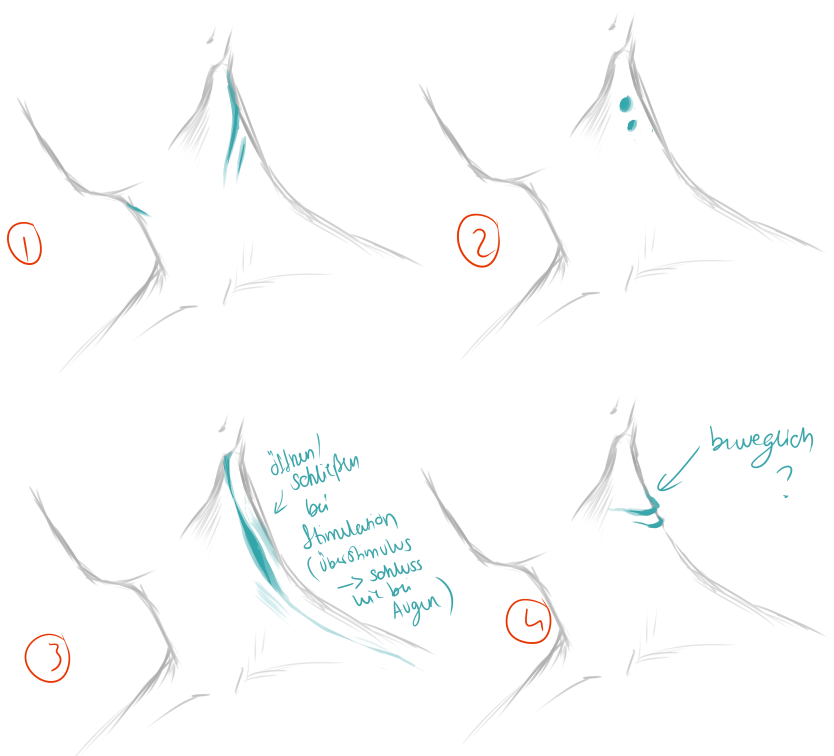
\includegraphics[width=0.7\linewidth]{Abbildungen/Weltenbau/Lebensformen/Sinnesorgan_Auswahl}
	\caption[mögliche Form des Sinnesorgans]{Die möglichen Formen eines Sinnesorgans zum Spüren von Magie.}
	\label{fig:sinnesorganauswahl}
\end{figure}

\subsubsection{Dunkles Volk}

\subsubsection{Zwerge} \label{rasse:zwerge}


\subsubsection{Halblinge} \label{rasse:halblinge}

\subsubsection{Sylvan} \label{rasse:sylvan}
\begin{itemize}
	\item diese Menschenart lebt in dem \npref{formation:gigantus}, wo die Bäume so hoch werden, dass wir im Vgl. so groß wie Mäuse oder Käfer sind
	\item Sie leben auf den Ebenen über dem Boden, wo die riesigen Äste der Bäume neue Ebenen erschaffen. Seltenst betreten sie den Waldboden
	\item ein Ritual könnte sein, dass sie die Leichen der Toten in Ast- und Blattwiegen aufbahren und sie dann  Richtung Erdboden schicken
	\item sie sind etwas größer als normale Menschen (Durchschnitt 15 cm größer), sind deutlich dünner und bewegen sich sehr grazil
	\item aufgrund des extremen Vorteils der Fähigkeit, Druck bzw Wind zu beeinflussen, ebenso wie die Atombindungen zu verhärten; aufgrund dessen haben diese Allele alle anderen verdrängt und man findet bei dieser Menschenart keine andere Magienutzung mehr
	\item eine ihrer Anpassungen an den Lebensraum: der Schwanz. Sie haben den Schwanz wieder rückentwickelt, weil der sehr stark bei der Stabilisation des Gleichgewichts hilft, was in den luftigen Höhen des Lebensraums von starkem Vorteil ist
\end{itemize}


\subsection{Tiere}
\subsubsection{Echte Tiere}
\paragraph{Regenbogen Oktopus} Könnte tatsächlich eine Inspiration für Meerjungfrauen gewesen sein (insbes. Start des Videos): \href{https://img-9gag-fun.9cache.com/photo/aVYpQVK\_460svvp9.webm}{9gag.com}
\paragraph{Axolotl} Sind einfach süß. Wir wollen sie dabei haben!

\subsection{Pflanzen}
\subsubsection{Echte Pflanzen}
\paragraph{Sandbüchsenbaum} \href{https://de.wikipedia.org/wiki/Sandb\%C3\%BCchsenbaum}{Wikipedia}. Die Stacheln des Baumes sind voller Gift. Die Früchte sehen wie kleine Kürbisse aus und wenn sie reif sind, explodieren sie und schleudern die Samen mit bis zu 240 km/h weg.

\subsection{Mikroorganismen}